\section{Transforming For Improved Fit}
This section provides a different interpretation of DAWIT, the metric learning
algorithm presented in Section 4.1.
We start by introducing Fit-Improving Iterative Representation Adjustment
(FIIRA), a function approximation framework under which DAWIT falls.
We then present an intuitive explanation of the rational behind DAWIT.

\subsection{Fit-Improving Iterative Representation Adjustment}
The problem statement of curve-fitting is as follows: given a set of training
points, $D = \{(x_i,y_i)\ |\ i = 1, \ldots, n\}$, of point-value pairs with
$y_i = f(x_i)$ for some function $f : X \to \mathbb{R}$,
produce a function $\tilde f$ to approximate $f$ well, for some measure of
approximation quality.

A regressor, $r$, is a procedure for creating fits from some space of
functions, $\mathcal{F}_r$.
If $f$ is not well approximated by any function in $\mathcal{F}_r$,
the fit generated by $r$ is guaranteed to be poor.
One way to fix to this problem is to transform the domain of $f$ and work in a
space where $f$ \textit{is} well approximated. Choosing such a transform
requires prior knowledge or assumptions about $f$.

Since we are not in a position to make assumptions about $f$,
we wish to infer a transform directly from the data.
Our idea for doing so, is to pass $D$ to the regressor,
then use the approximation produced to infer a transform $\Phi$ of the
domain $X$ such that $f$ on $\Phi(X)$ is better approximated by $\mathcal{F}_r$.
Algorithm 1 describes the framework for doing this.
The procedure takes as input a dataset, $D$; a regressor, $REGR$;
and a transform generator, $TF$.

\begin{algorithm}
\caption{Fit-Improving Iterative Representation Adjustment}\label{FIIRA}
\begin{algorithmic}[1]
\Procedure{FIIRA}{$D,\ REGR,\ TF$}
	\State $\Phi_0 \gets x \mapsto x$
          \Comment{Identity transform}
        \State $D_0 \gets D$
	\State $i \gets 0$
	\Repeat
		\State $\tilde f_{i+1} \gets REGR(D_i)$
                  \Comment{Perform regression}
		\State $\Phi_{i+1}\gets TF(\tilde f_{i+1}, D_i)$
                  \Comment{Produce transform}
                \State $D_{i+1} \gets \{(\Phi_{i+1}(x), y)\ |\ (x,y) \in D_{i}\}$
                  \Comment{Update the dataset}
		\State $i \gets i+1$
	\Until{$\tilde f_{i} \approx \tilde f_{i-1}}$
           \Comment{Or until best fit attained}
	\State \textbf{return} $x \mapsto \tilde f_{i}(\Phi_{i-1}(x))$
\EndProcedure
\end{algorithmic}
\end{algorithm}

A formal analysis of the properties of FIIRA
for a general regression scheme and transform generator
is outside the scope of this paper and is left for future work.
What follows is a discussion of FIIRA for the special
case where the regressor is a local-averaging kernel smoother
and the transform generator is DAWIT.

\subsection{Dimension-Adding Wrinkle-Ironing Transform}
In the paper we claim that the metric created by DAWIT corresponds to a
transform that warps the state space through a higher dimension.
We now elaborate on that.

Consider a transform generator that, given a function $f$ with domain $X$, 
returns a transform $\Phi$ which maps every $x \in X$ to $\langle x | f(x)\rangle$
(the bar represents concatenation).
$\Phi$ stretches $X$ into $d+1$ dimensions in a way that
pulls apart points that differ in value (See Figure 6).

\begin{figure}[!htb]
  \minipage{0.5\textwidth}
    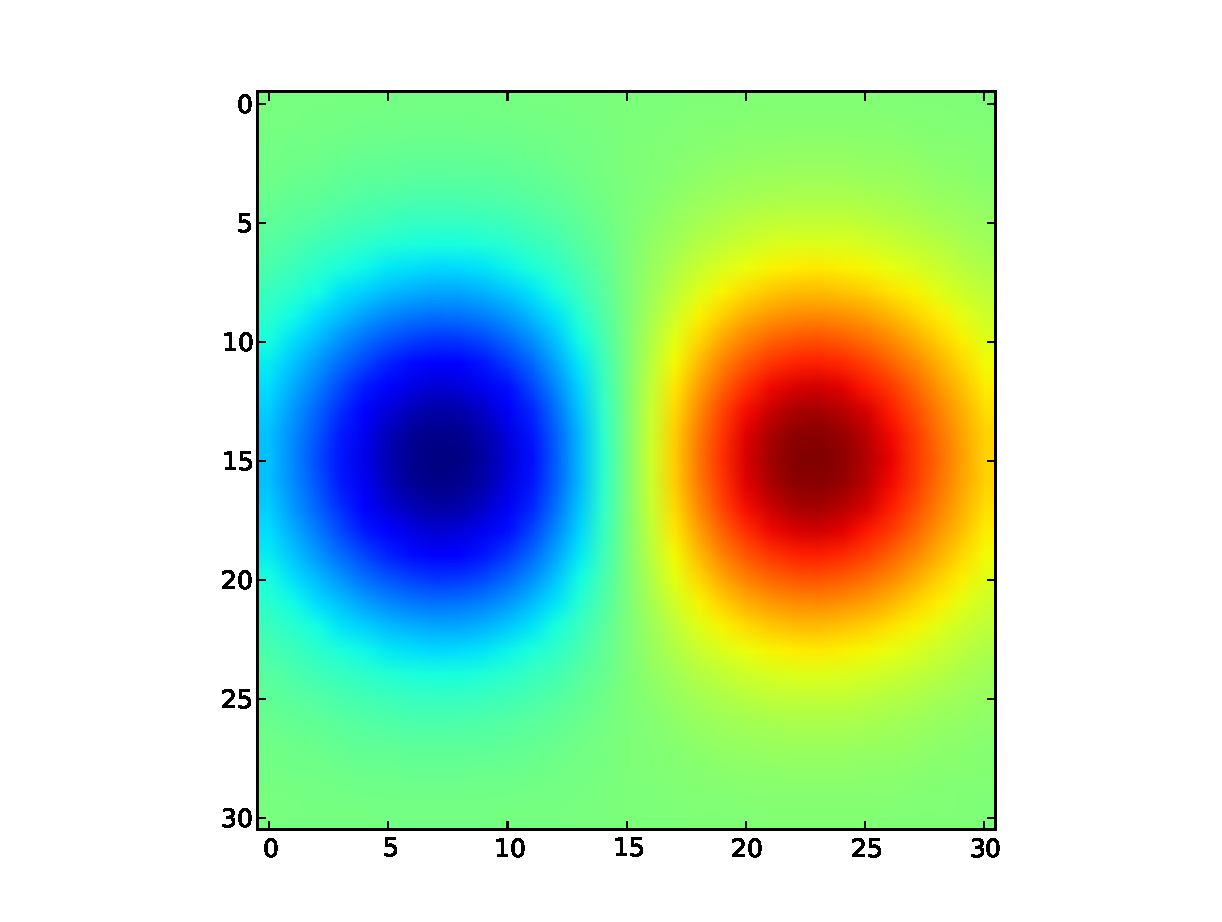
\includegraphics[width=\linewidth]{../writeup/figs/bumps.pdf}
  \endminipage\hfill
  \minipage{0.5\textwidth}
    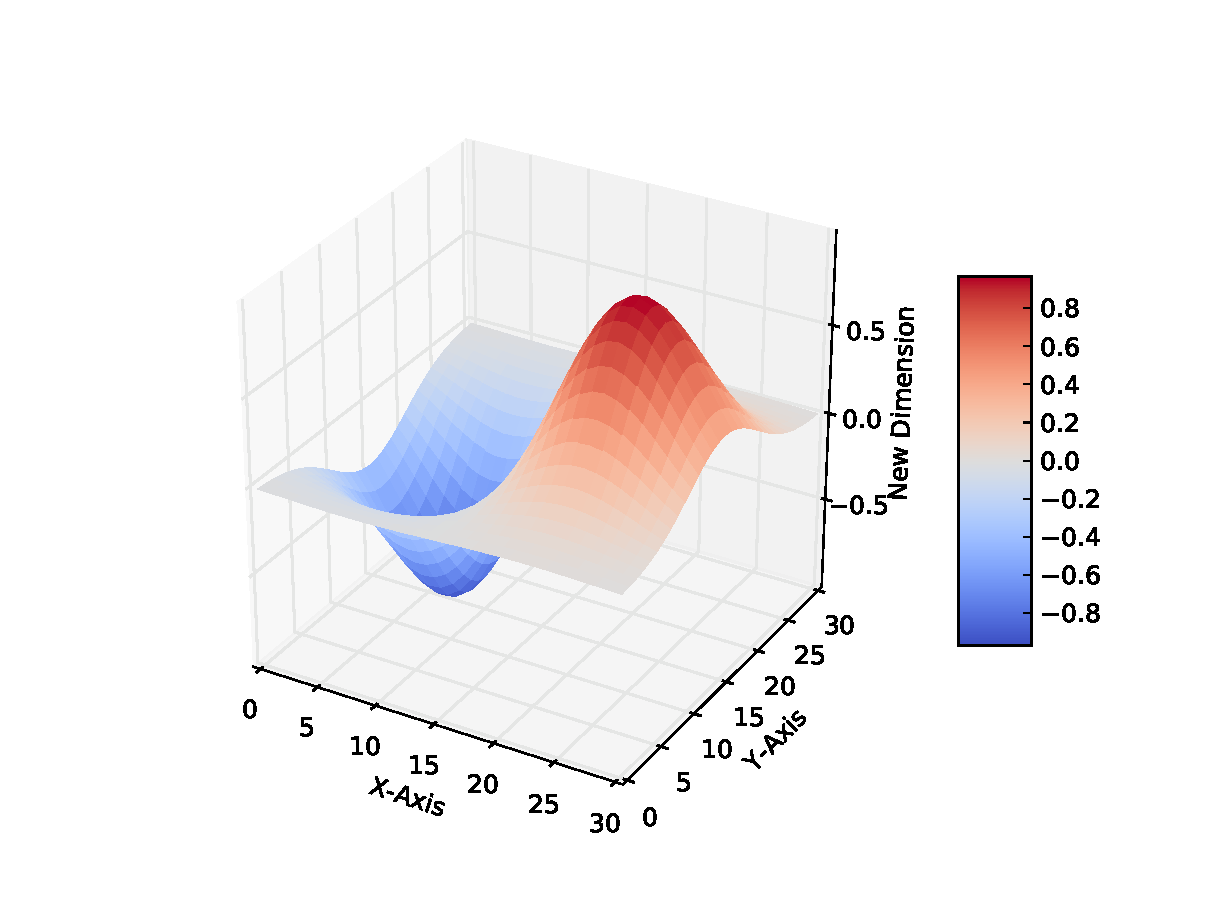
\includegraphics[width=\linewidth]{../writeup/figs/tfbumps.pdf}
  \endminipage
   \label{dimad}
\caption[Dimension-Adding WIT example]
{The figure on the left is a heatmap of some function with a two-dimensional
domain.
The areas in red are where it attains a high value and the ones in blue
are where it attains a low value.
The figure on the right shows the two-dimensional domain stretched through three
dimensional space in such a way that separates points that differ in value.
The red areas are pulled up and out of the page while the blue ones are pushed
down and into the page.
Distances in this transformed space correspond to the metric produced by DAWIT.}
\end{figure}

After the transformation, the distance between two points $a$ and $b$ in the
domain of $f$ becomes
$$\|\Phi(a)- \Phi(b)\| = \sqrt{\|a-b\|^2 + (f(a) - f(b))^2}.$$
Note that $\|\Phi(a)- \Phi(b)\|$ varies more closely with $|f(a) - f(b)|$
than does $\|a-b\|$.

The transform $\Phi$ does what we want, but it has two problems;
 it is sensitive to the scale of $f$, and it can change the diameter of $X$.
We fix these problems by normalizing $f$ by $\alpha\mu_f$ and $\Phi(X)$ by $c_0$
(as defined in the main body of the paper).

With these two changes, $\Phi$ maps the $m$-dimensional vector, $x = (x_1, \ldots, x_m)$
to the $m+1$-dimensional $x' = (c_0x_1, \ldots, c_0x_m, c_0\alpha\mu_f\cdot f(x))$.
The distance metric that corresponds to the final form of this transform is
 $$\|\Phi(a)- \Phi(b)\| = c_0 \sqrt{ \|a-b\|^2 + \alpha^2\mu_f^2\cdot(f(a) - f(b))^2}.$$
When we substitute for $\mu_f$ and $c_0$, this equals the metric produced by DAWIT;
hence the name ``dimension-adding'' VCPM relaxation.
We refer to kernel regression augmented to use DAWIT as FDK because it is a
\textbf{F}IIRA approach combining \textbf{D}AWIT and \textbf{K}ernel-regression.


\subsection{How DAWIT works}
Kernel-regression produces function estimates using local averaging.
As a result, the approximation is good where the target function, f,
is linear and bad where it has high curvature. It follows that the
curvature of the estimate, $h(x)$, is correlated with the approximation
error. Thus, we can infer where the approximation likely to be poor
just by looking at the approximation.

We use this insight to construct a transform of the input domain, $X$,
into a space where $h$ (and thus also $f$) are smoother. Our transform
warps the $m$ dimensional $X$ into the $m+1$ dimensional $X'$ in such a way
that its diameter is preserved but some neighborhoods grow or shrink
depending on the slope of $h$. The metric produced by DAWIT corresponds
to distances in $X'$.

Let $f$ be the unit step function and let $X = [-1,1]$. One iteration of
kernel regression produces $h$ resembling a sigmoid. $h$ attains its maximum
slope near $x=0$. Performing DAWIT with $h$ produces a metric, $d$, that
stretches the area around $x=0$ (i.e. $d(-\epsilon, \epsilon) > 2*\epsilon$,
for small $|\epsilon|$) and squashes the regions near $x=1$ and $x=-1$. The
point $x=0$ itself may get moved closer to $x=1$ or $x=-1$, but that
does not matter. What matters is that on the next round of regression
the region around $x=0$ is magnified, making it easier to pinpoint where
the discontinuity lies. This magnification is analogous to using a smaller bandwidth at $x=0$.

One can see now why we call the transform "wrinkle-ironing".
The discontinuity in the step function resembles a crease on an article of clothing.
Repeated application of the transform smooths this and similar value cliffs
much like a hot iron passing over a wrinkly shirt.

\subsection{Value Consistent Pseudometric}
In the main body of the paper, we claimed that using the VCPM as a valid
metric in kernel regression was theoretically sound. We now justify that claim.

When viewed under the lens of a FIIRA approach, the VCPM can be seen as coming
from a transform $\Phi^*$ that satisfies $\|\Phi^*(x)- \Phi^*(x')\| = \mu_f |f(x) - f(x')|$.
A transform that satisfies this property is $\Phi^*(x) = \mu_f f(x)$.
Under this interpretation, we are mapping each point to its scaled value
and performing kernel regression to fit a line.
Only points with identical values get mapped to the same point by the transform.
Since $\Phi^*$ is a safe to use before doing regression,
performing kernel regression with the VCMP for the function being approximated
cannot cause problems.

\clearpage
